\chapter{Results}

I analysed three consecutive networks, each aggregated for ten hours starting at 8am. The age distribution for each network is shown in figure~\ref{fig:ages}.

\begin{figure}[htb]
	\centering
	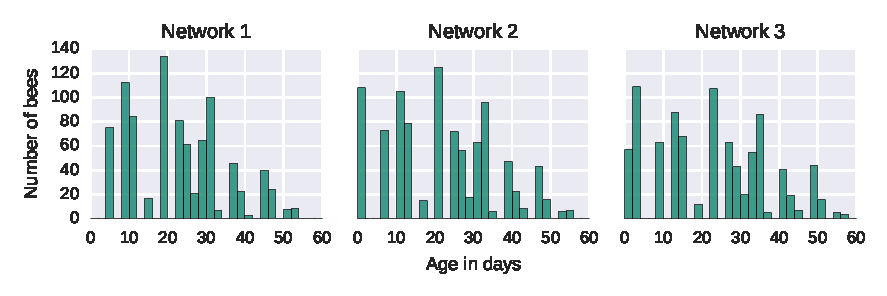
\includegraphics[width=1.0\textwidth]{Figures/ages}
	\caption[Distribution of gge per Network]{Distribution of age per network.}
	\label{fig:ages}
\end{figure}


\section{Static Network Analysis}

The three networks consist of 1000 nodes with a density of about 60\%. The diameter is three for all the networks. The average shortes path length is inbetween 1 and 2. 

\begin{table}
\centering
\begin{tabular}{lrrr}
\toprule
{} &        \#4 &        \#5 &        \#6 \\
\midrule
Date             &     2016-08-20 &     2016-08-22 &     2016-08-24 \\
$N$            &      922 &      978 &      922 \\
$L$            &   291179 &   256066 &   259421 \\
$D$          &     0.69 &     0.54 &     0.61 \\
$\langle d_{\texttt{max}} \rangle$         &        3 &        3 &        3 \\
$\langle d \rangle$ &     1.32 &     1.46 &     1.39 \\
$C_\Delta$              &     0.79 &     0.72 &     0.75 \\
$ \langle k \rangle$       &   631.62 &   523.65 &   562.74 \\
$ \langle s \rangle$       &  5680.17 &  3977.94 &  4205.99 \\
$k_{\texttt{max}}$           &      850 &      822 &      842 \\
$s_{\texttt{max}}$          &    13555 &    10468 &    10864 \\
 $k_{\texttt{min}}$           &        1 &        3 &       51 \\
$s_{\texttt{min}}$          &        1 &        8 &       64 \\
\bottomrule
\end{tabular}
\caption{Some table caption: Soem text here}
\label{tab:stats}
\end{table}

\begin{figure}[htb]
	\centering
	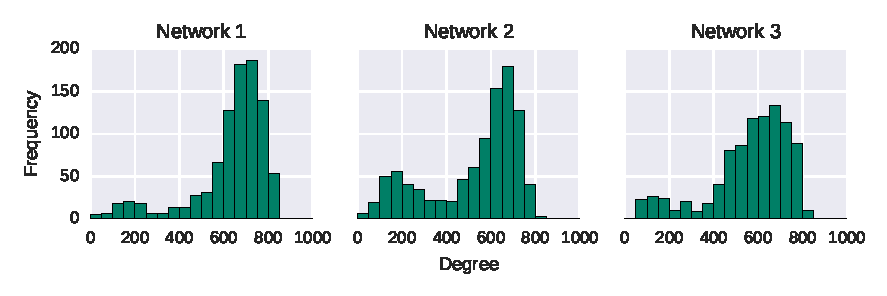
\includegraphics[width=1.0\textwidth]{Figures/stat-degreeDist}
	\caption[Degree Distribution]{Degree Distribution}
	\label{fig:statDegreeDist}
\end{figure}


\begin{figure}[htb]
	\centering
	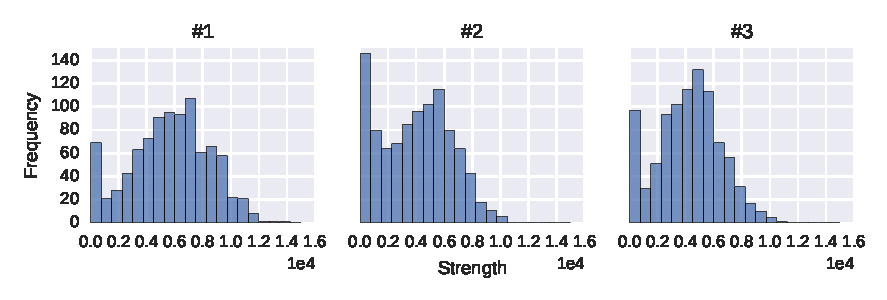
\includegraphics[width=1.0\textwidth]{Figures/stat-strengthDist}
	\caption[Strength Distribution]{Strength Distribution: Weighted Degree Distribution}
	\label{fig:statStrengthDist}
\end{figure}

\begin{figure}[htb]
	\centering
	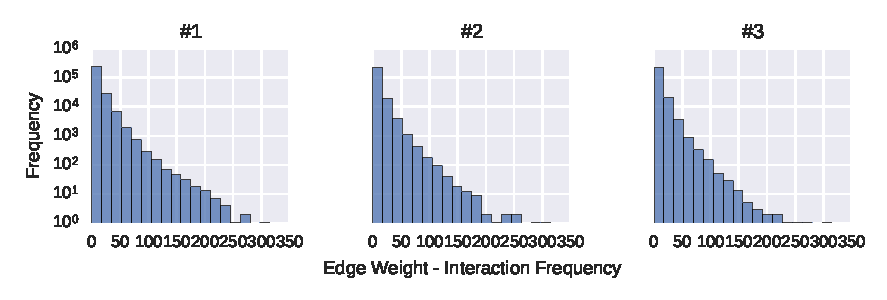
\includegraphics[width=1.0\textwidth]{Figures/stat-edgeWeightDist}
	\caption[Edge Weight Distribution]{Edge Weight Distribution - Edge weight is the contact frequency}
	\label{fig:statEdgeWeightDist}
\end{figure}


\begin{figure}[htb]
	\centering
	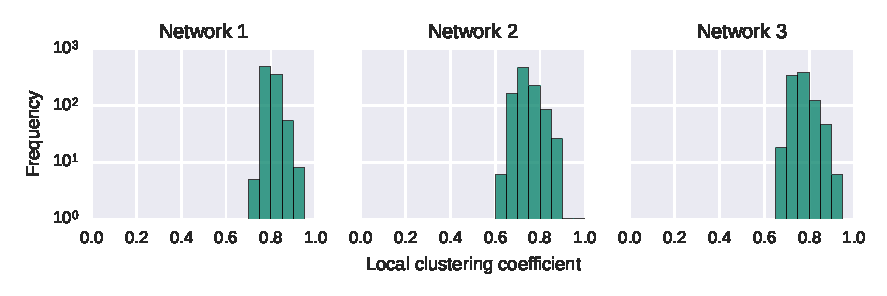
\includegraphics[width=1.0\textwidth]{Figures/stat-lccDist}
	\caption[Local clustering coefficien]{Local clustering coefficien - unweighted}
	\label{fig:lccDist}
\end{figure}


\subsection{Centrality Measures}
Weglassen.



\section{Community Detection}

Using the leading eigenvector community detection algorithm revealed in seven networks two communities with about the same number of nodes and in two networks three communities. The first community contains the queen and on average younger bees than the second (and third) community.

The Kolmogorov–Smirnov  test ($p=7.2e^{-10} \pm2.6e^{-9}$) shows that for each network, the are distributions are significantly different. [TODO: wie schreibt man das?]

\begin{table}
\centering
\begin{tabularx}{0.8\textwidth}{lccrrr}
	\toprule
	{} & Date & \#Members & Proportion & Age & SD\\
	\midrule
	\#0 & 2016-08-13 & 673     & 54.14\% & $22.08$ & $\pm17.10$ \\
	  &            & $570^*$ & 45.86\% & $9.95$ & $\pm14.26$ \\
	\midrule 
	\#1 & 2016-08-14 & 502     & 42.08\% & $24.21$ & $\pm15.05$ \\
	  &			   & $354^*$ & 29.67\% &  $8.26$ & $\pm14.73$ \\
	  &			   & 337     & 28.25\% & $17.57$ & $\pm18.64$ \\
	\midrule     
	\#2 & 2016-08-16 & $481^*$ & 41.22\% & $10.44$ & $\pm15.18$ \\
	  &		       & 471     & 40.36\% & $24.82$ & $\pm16.26$ \\
	  &		       & 215     & 18.42\% & $20.11$ & $\pm17.93$ \\
	\midrule  
	\#3 & 2016-08-17 & 639     & 58.36\% & $23.62$ & $\pm18.25$ \\
	  &            & $456^*$ & 41.64\% & $11.75$ & $\pm14.18$ \\
	\midrule   
	\#4 & 2016-08-20 & 488     & 52.93\% & $25.15$ & $\pm19.49$ \\
	  &            & $434^*$ & 47.07\% & $16.81$ & $\pm17.91$ \\
	\midrule   							
	\#5 & 2016-08-22 & $503^*$ & 51.43\% & $15.44$ & $\pm19.54$ \\
	  &            & 475     & 48.57\% & $26.37$ & $\pm18.01$ \\
	\midrule  
	\#6 & 2016-08-24 & 537     & 58.24\% & $27.26$ & $\pm17.84$ \\
	  &            & $385^*$ & 41.76\% & $12.85$ & $\pm20.24$ \\
	\midrule  
	\#7 & 2016-08-25 & 455     & 58.11\% & $27.35$ & $\pm19.70$ \\
	  &            & $328^*$ & 41.89\% & $11.81$ & $\pm19.28$ \\
	\midrule 
	\#8 & 2016-09-02 & $198^*$ & 52.24\% & $19.32$ & $\pm26.44$ \\
	  &            & 181     & 47.76\% & $30.59$ & $\pm27.25$ \\
	\bottomrule
\end{tabularx}
\caption{Some table caption: Community indicated with * contains the queen.}
\label{tab:communities}
\end{table}

\begin{figure}[htb]
	\centering
	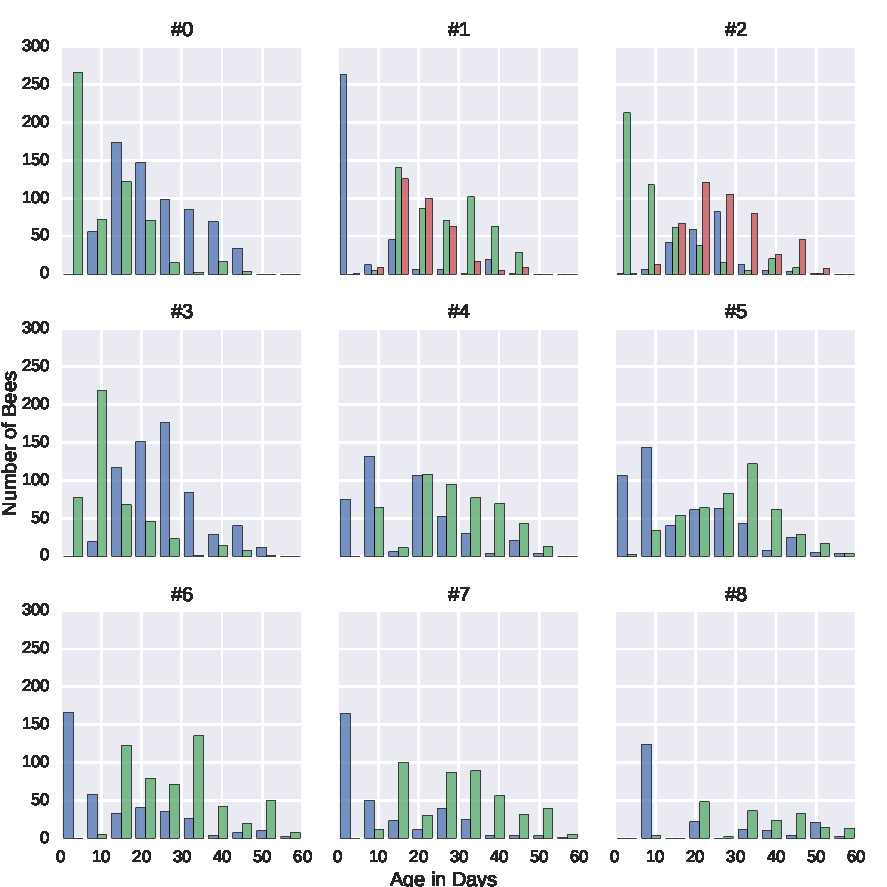
\includegraphics[width=1.0\textwidth]{Figures/ageDistribution}
	\caption{Distribution of age per community for each network}
	\label{fig:ageDist}
\end{figure}


\subsubsection{Age Distribution}

\subsubsection{Spatial Distribution}
